\section{Lognormal Distribution ($\text{Lognormal}(\mu ,\sigma ^{2})$, $LN(\mu ,\sigma ^{2})$)}

\begin{table}[H]
    \hfill
    \begin{minipage}{0.45\linewidth}
        \begin{figure}[H]
            \centering
            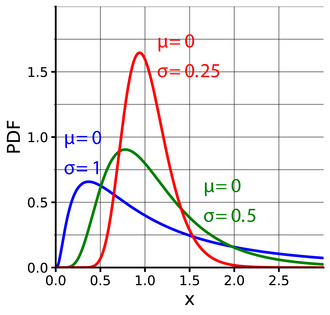
\includegraphics[
                width=\linewidth,
                height=5cm,
                keepaspectratio,
            ]{images/distributions/Log-normal-pdfs.png}
            \caption{Lognormal Distribution: PDF \cite{wiki/Log-normal_distribution}}
        \end{figure}
    \end{minipage}
    \hfill
    \begin{minipage}{0.45\linewidth}
        \begin{figure}[H]
            \centering
            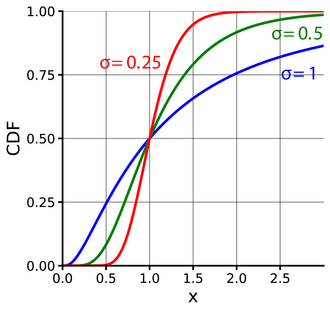
\includegraphics[
                width=\linewidth,
                height=5cm,
                keepaspectratio,
            ]{images/distributions/Log-normal-cdfs.png}
            \caption{Lognormal Distribution: CDF \cite{wiki/Log-normal_distribution}}
        \end{figure}
    \end{minipage}
    \hfill
\end{table}



\subsection{PDF}

\begin{enumerate}
    \item[] $
        f_L(x)
        = f_{\mu, \sigma}(x)
        = \dfrac{1}{x\sigma \sqrt{2\pi}} \exp\dCurlyBrac{
            -\dfrac{(\log(x) - \mu)^2}{2\sigma^2}
        }
        = \dfrac{1}{x\sigma} \phi\dParenBrac{\dfrac{\log(x) - \mu}{\sigma}}
    $
    \hfill \cite{statistics/book/Statistics-for-Data-Scientists/Maurits-Kaptein}

    \item the lognormal PDF describes populations with positive values
    \hfill \cite{statistics/book/Statistics-for-Data-Scientists/Maurits-Kaptein}

    \item relative standard deviation  is constant for the lognormal PDF.
    This means that larger values demonstrate larger variability, but the ratio with variability is constant whether we observe smaller or larger values.
    \hfill \cite{statistics/book/Statistics-for-Data-Scientists/Maurits-Kaptein}

    \item the lognormal PDF is not symmetric like the normal PDF, which makes sense when values are limited from below, but not from above.
    \hfill \cite{statistics/book/Statistics-for-Data-Scientists/Maurits-Kaptein}

    \item  If the population values can be described by a lognormal PDF, the normal PDF would then describe the logarithmic transformation of the population values (using the natural logarithm).
    \hfill \cite{statistics/book/Statistics-for-Data-Scientists/Maurits-Kaptein}

    \item The parameters $\mu$ and $\sigma$ have a different meaning in the lognormal PDF than in the normal PDF.
    They do represent the population mean and standard deviation, but only for the logarithmic transformed values of the population.
    Their meaning in relation to the mean and standard deviation of the population values in the original scale is now more complicated.
    \hfill \cite{statistics/book/Statistics-for-Data-Scientists/Maurits-Kaptein}
\end{enumerate}






\subsection{Summary}

\begin{enumerate}
    \item \textbf{Notation}:
    ${\displaystyle \operatorname {Lognormal} \left(\mu ,\,\sigma ^{2}\right)}$
    OR
    $\mathcal{L N} (\mu, \sigma^2)$
    \hfill \cite{wiki/Log-normal_distribution, statistics/book/Statistics-for-Data-Scientists/Maurits-Kaptein}

    \item \textbf{Parameters}:
    \begin{enumerate}
        \item ${\displaystyle \mu \in (-\infty ,+\infty )}$: logarithm of location
        \hfill \cite{wiki/Log-normal_distribution, statistics/book/Statistics-for-Data-Scientists/Maurits-Kaptein}

        \item ${\displaystyle \sigma >0}$: logarithm of scale
        \hfill \cite{wiki/Log-normal_distribution, statistics/book/Statistics-for-Data-Scientists/Maurits-Kaptein}
    \end{enumerate}

    \item \textbf{Support}: ${\displaystyle x\in (0,+\infty )}$
    \hfill \cite{wiki/Log-normal_distribution, statistics/book/Statistics-for-Data-Scientists/Maurits-Kaptein}

    \item \textbf{PDF}:
    ${\displaystyle {\dfrac {1}{x\sigma {\sqrt {2\pi }}}}\exp \left(-{\dfrac {\left(\ln x-\mu \right)^{2}}{2\sigma ^{2}}}\right)}$
    \hfill \cite{wiki/Log-normal_distribution, statistics/book/Statistics-for-Data-Scientists/Maurits-Kaptein}

    \item \textbf{CDF}:
    $
        {\displaystyle {{\dfrac {1}{2}}\left[1+\operatorname {erf} \left({\dfrac {\ln x-\mu }{\sigma {\sqrt {2}}}}\right)\right]
        =\Phi {\left({\dfrac {\ln x-\mu }{\sigma }}\right)}}}
    $
    \hfill \cite{wiki/Log-normal_distribution}

    \item \textbf{Quantile}:
    $
        {\displaystyle {\exp \left(\mu +{\sqrt {2\sigma ^{2}}}\operatorname {erf} ^{-1}(2p-1)\right)
        =\exp(\mu +\sigma \Phi ^{-1}(p))}}
    $
    \hfill \cite{wiki/Log-normal_distribution}

    \item \textbf{Mean}: ${\displaystyle \exp \left(\mu +{\dfrac {\sigma ^{2}}{2}}\right)}$
    \hfill \cite{wiki/Log-normal_distribution}

    \item \textbf{Median}: ${\displaystyle \exp(\mu )}$
    \hfill \cite{wiki/Log-normal_distribution}

    \item \textbf{Mode}: ${\displaystyle \exp \left(\mu -\sigma ^{2}\right)}$
    \hfill \cite{wiki/Log-normal_distribution}

    \item \textbf{Variance}:
    ${\displaystyle \left[\exp(\sigma ^{2})-1\right]\exp \left(2\mu +\sigma ^{2}\right)}$
    \hfill \cite{wiki/Log-normal_distribution}

    \item \textbf{Skewness}:
    ${\displaystyle \left[\exp \left(\sigma ^{2}\right)+2\right]{\sqrt {\exp(\sigma ^{2})-1}}}$
    \hfill \cite{wiki/Log-normal_distribution}

    \item \textbf{Excess kurtosis}:
    ${\displaystyle \exp \left(4\sigma ^{2}\right)+2\exp \left(3\sigma ^{2}\right)+3\exp \left(2\sigma ^{2}\right)-6}$
    \hfill \cite{wiki/Log-normal_distribution}

    \item \textbf{Entropy}: ${\displaystyle \log _{2}\left({\sqrt {2\pi e}}\,\sigma e^{\mu }\right)}$
    \hfill \cite{wiki/Log-normal_distribution}

    \item \textbf{Fisher information}:
    ${\displaystyle {\dfrac {1}{\sigma ^{2}}}{\begin{pmatrix}1&0\\0&2\end{pmatrix}}}$
    \hfill \cite{wiki/Log-normal_distribution}

    \item \textbf{Method of moments}:
    \begin{enumerate}
        \item ${\displaystyle \mu =\ln \operatorname {E} [X]-{\dfrac {1}{2}}\ln \left({\dfrac {\operatorname {Var} [X]}{\operatorname {E} [X]^{2}}}+1\right),}$
        \hfill \cite{wiki/Log-normal_distribution}

        \item ${\displaystyle \sigma ={\sqrt {\ln \left({\dfrac {\operatorname {Var} [X]}{\operatorname {E} [X]^{2}}}+1\right)}}}$
        \hfill \cite{wiki/Log-normal_distribution}
    \end{enumerate}

    \item \textbf{Expected shortfall}:
    $
        {\displaystyle {{\dfrac {e^{\mu +{\dfrac {\sigma ^{2}}{2}}}}{2p}}\left[1+\text{erf} \left({\dfrac {\sigma }{\sqrt {2}}}+\operatorname {erf} ^{-1}(2p-1)\right)\right]
        ={\dfrac {e^{\mu +{\dfrac {\sigma ^{2}}{2}}}}{1-p}}\left[1-\Phi (\Phi ^{-1}(p)-\sigma )\right]}}
    $
    \hfill \cite{wiki/Log-normal_distribution}

    \item \textbf{Relative Standard Deviation}: $\sqrt{\exp\dCurlyBrac{\sigma^2} - 1}$
    \hfill \cite{statistics/book/Statistics-for-Data-Scientists/Maurits-Kaptein}
    \\
    (RSD = standard deviation divided by the mean)
    \hfill \cite{statistics/book/Statistics-for-Data-Scientists/Maurits-Kaptein}
\end{enumerate}





\subsection{Lognormally Distributed Populations}

\begin{enumerate}
    \item If $X$ is lognormally $\mathcal{L N} (\mu, \sigma^2)$ distributed then $\log(X)$ is normal $\mathcal{N} (\mu, \sigma^2)$.
    \hfill \cite{statistics/book/Statistics-for-Data-Scientists/Maurits-Kaptein}

    \item If $X_1 , X_2, \cdots , X _n$ are i.i.d. lognormally distributed, the sample average and sample variance of the transformed random variables $\log (X_1),\ \log (X_2) , \cdots , \log (X_ n )$, with log the natural logarithm, are given by
    $
        \bar{X}_{\log} = \dfrac{1}{n} \dsum^n _{i=1} \log (X _i )
    $
    and
    $
        S^2 _{\log} = \dfrac{1 }{n - 1} \dsum^n _{i=1} (\log (X _i ) - \bar{X}_{\log} )^2
    $
    \hfill \cite{statistics/book/Statistics-for-Data-Scientists/Maurits-Kaptein}

    \item These sample statistics are \textbf{unbiased estimates} of $\mu$ and $\sigma^ 2$ , respectively.
    \hfill \cite{statistics/book/Statistics-for-Data-Scientists/Maurits-Kaptein}

    \item The distribution function of $\bar{X}_{\log}$ is normally distributed $\mathcal{N} \dParenBrac{\mu, \dfrac{\sigma ^ 2}{n}}$ and $\dfrac{(n - 1) S^2 _{\log}}{\sigma ^ 2}$ has a chi-square distribution function with $n - 1$ degrees of freedom.
    \hfill \cite{statistics/book/Statistics-for-Data-Scientists/Maurits-Kaptein}

    \item the geometric average $\exp ( \bar{X}_{\log} ) = \dprod ^n _{i=1} \sqrt[n]{{X}_ i}$ is lognormally distributed.
    \hfill \cite{statistics/book/Statistics-for-Data-Scientists/Maurits-Kaptein}
\end{enumerate}





\subsection{Method of Moments Estimation (MME)}

\begin{enumerate}
    \item consider the random variable $X$ that is lognormally distributed, i.e. $X \sim \mathcal{LN} (\mu ,\sigma ^{2})$
    \hfill \cite{statistics/book/Statistics-for-Data-Scientists/Maurits-Kaptein}

    \item The PDF ($f_L$) contains only two parameters $\theta_1 = \mu$ and $\theta_2 = \sigma^ 2 $
    \hfill \cite{statistics/book/Statistics-for-Data-Scientists/Maurits-Kaptein}

    \item we only need to solve the two equations:
    \hfill \cite{statistics/book/Statistics-for-Data-Scientists/Maurits-Kaptein}
    \begin{enumerate}
        \item $M_1 = \bar{X} = \mu  ( f_ L ) = \exp (\mu  + 0.5 \sigma  ^2)$
        \hfill \cite{statistics/book/Statistics-for-Data-Scientists/Maurits-Kaptein}

        \item $M_2 = \sigma  ^2 ( f _L ) = \exp (2\mu  + \sigma ^ 2)\ (\exp (\sigma  ^2) - 1)$
        \hfill \cite{statistics/book/Statistics-for-Data-Scientists/Maurits-Kaptein}
    \end{enumerate}

    \item using $\dfrac{\sigma ^2 ( f_ L )}{\mu^2 ( f_ L )} = \exp (\sigma^ 2) - 1$, we obtain that $\sigma^ 2$ can be estimated by
    \hfill \cite{statistics/book/Statistics-for-Data-Scientists/Maurits-Kaptein}
    \\
    .\hfill
    $
        \tilde{\sigma}^ 2
        = \log \dParenBrac{ 1 + \dfrac{M_2} {\bar{X}^2} }
        = \log ( \bar{X}^2 + M_2 ) - 2 \log ( \bar{X} )
    $
    \hfill \cite{statistics/book/Statistics-for-Data-Scientists/Maurits-Kaptein}

    \item Using the estimator $\tilde{\sigma} ^2$, we obtain the moment estimator for $\mu$, which is given by
    \hfill \cite{statistics/book/Statistics-for-Data-Scientists/Maurits-Kaptein}
    \\[0.2cm]
    .\hfill
    $
        \mu
        = \log ( \bar{X}) - 0.5 [\log ( \bar{X}^2 + M_2 ) - 2 \log ( \bar{X} )]
        = 2 \log ( \bar{X} ) - 0.5 \log ( \bar{X}^2 + M_2 )
    $
    \hfill \cite{statistics/book/Statistics-for-Data-Scientists/Maurits-Kaptein}

    \item \textbf{alternative approach}: consider the set of transformed random variables $\log (X_1), \log (X_2) , \cdots , \log (X _n )$.
    \hfill \cite{statistics/book/Statistics-for-Data-Scientists/Maurits-Kaptein}
    \begin{enumerate}
        \item These random variables are normally distributed with mean $\mu$ and variance $\sigma^ 2$.
        \hfill \cite{statistics/book/Statistics-for-Data-Scientists/Maurits-Kaptein}

        \item The moment estimators in this setting are now $\tilde{\mu} = \bar{X}_{\log}$ and $\tilde{\sigma}^ 2 = \dfrac{n - 1}{n}S^2 _{\log}$, where $\bar{X}_{\log}$ and $S^2 _{\log} $.
        \hfill \cite{statistics/book/Statistics-for-Data-Scientists/Maurits-Kaptein}
    \end{enumerate}

\end{enumerate}





\subsection{Maximum Likelihood Estimation (MLE)}

\begin{enumerate}
    \item the set of parameters that we want to estimate is given by $\theta_1 = \mu$ and $\theta_2 = \sigma^ 2 $.
    \hfill \cite{statistics/book/Statistics-for-Data-Scientists/Maurits-Kaptein}

    \item The log likelihood in this setting is equal to
    \hfill \cite{statistics/book/Statistics-for-Data-Scientists/Maurits-Kaptein}
    \\
    .\hfill
    $
        \dsum ^n _{i=1} \log f _L (X_i )
        = \dsum ^n _{i=1} \dParenBrac{
            - \dfrac{(\log (X_i ) - \mu)^2} {2\sigma^2}
            - \log (\sqrt{2\pi})
            - \log(X_i )
            - \log (\sigma )
        }
    $
    \hfill \cite{statistics/book/Statistics-for-Data-Scientists/Maurits-Kaptein}

    \item The terms log $\sqrt{2\pi}$ and $\log(X_i )$ can essentially be ignored, since they will be the same whatever we choose for $\mu$ and $\sigma$.
    \hfill \cite{statistics/book/Statistics-for-Data-Scientists/Maurits-Kaptein}

    \item Taking the derivatives with respect to $\mu$ and $\sigma$ and equating them to zero we obtain the following equations
    \hfill \cite{statistics/book/Statistics-for-Data-Scientists/Maurits-Kaptein}
    \\
    .\hfill
    $
        \dsum^n_{i=1} \dParenBrac{ \dfrac{\log(X_i ) - \mu }{\sigma^ 2} } = 0
    $
    \hfill
    $
        \dsum ^n _{i=1} \dParenBrac{ \dfrac{(\log (X_i) - \mu)^2 }{\sigma^3} - \dfrac{1}{ \sigma}} = 0
    $
    \hfill \cite{statistics/book/Statistics-for-Data-Scientists/Maurits-Kaptein}

    \item Solving these equations leads to the solutions 
    \hfill \cite{statistics/book/Statistics-for-Data-Scientists/Maurits-Kaptein}
    \\
    .\hfill
    $\hat{\mu} = \bar{X}_{\log} = \dsum ^n _{i=1} \log(X_i ) $
    \hfill
    $
        \hat{\sigma}^ 2 
        = \dfrac{1}{n} \dsum^2 _{i=1}(\log(X_i ) - \bar{X}_{\log})^2 
        = \dfrac{n - 1}{n}S^2_{ \log}
    $
    \hfill \cite{statistics/book/Statistics-for-Data-Scientists/Maurits-Kaptein}

    \item These solutions are the MME of the logarithmically transformed random variables.
    This implies that the MLE for $\sigma^  2$ is not unbiased, since the expected value of $\hat{\sigma}^2$ is equal to $\mbbE[\hat{\sigma}^2] = \mbbE\dSquareBrac{\dfrac{n - 1}{n} S^2 _{\log}} = \dfrac{n - 1}{n} \sigma^2$, although this bias vanishes when the sample size gets large.
    \hfill \cite{statistics/book/Statistics-for-Data-Scientists/Maurits-Kaptein}

    \item Using the ML estimates for the density parameters to estimate the population parameters $\mu( f _L )$ or $\sigma^2( f_L )$ in the logarithm scale does not provide unbiased estimator for the mean of the population in the original scale, since the MLE estimate $\exp( \hat{\mu} + 0.5 \ \hat{\sigma}^2)$ is unequal to the expected value of the sample mean $\bar{X}$.
    \hfill \cite{statistics/book/Statistics-for-Data-Scientists/Maurits-Kaptein}

    
\end{enumerate}

















